% =====================================================================
% Sección: Experimentación y análisis de resultados
% Responsable: Parte 7 — Daniel Alonso Gracia Pinto
% Datos: resultados/resumen.csv, resultados/tabla_estadistica.csv y
%        resultados/comparacion_E2_vs_E1.csv (Parte 4).
% =====================================================================
\section{Experimentación y análisis de resultados}
\label{sec:experimentacion}

\subsection{Escenarios y ejecución}

Esta sección pone a prueba la hipótesis con los datos. Se ejecutaron los cuatro escenarios de la tabla~\ref{tab:escenarios} con los parámetros
de la tabla~\ref{tab:parametros}: E0 (sin movilidad), E1 (solo movilidad de nodo), E2
(solo movilidad de clúster) y E3 (ambas). E1, E2 y E3 se corrieron a las velocidades
$v \in \{1, 5, 10, 20\}$\,m/s y E0 una sola vez, cada configuración con diez réplicas
(\texttt{RngRun} $= 1, \dots, 10$): 130 corridas de 200\,s en total, todas completadas
sin errores y todas con paquetes recibidos. Las corridas se automatizaron con
\texttt{scripts/correr\_escenarios.sh}, las métricas se extrajeron de los XML de
FlowMonitor con \texttt{scripts/parse\_flowmon.py} y las tablas y figuras se generaron
con \texttt{scripts/graficar.py}.

Que un programa corra sin errores no garantiza que haga lo que se diseñó. Por eso,
antes del experimento, el programa se verificó con una batería de 46 pruebas
automáticas (\texttt{scripts/validar\_movilidad.py}). Las pruebas confirmaron que en E0
ningún nodo se mueve, que en E1 los CH permanecen fijos, que en E2 cada miembro conserva
exactamente su posición relativa a su CH, que clústeres y nodos no salen de sus regiones
($\pm 150$\,m y $\pm 40$\,m), que nunca se supera la velocidad configurada, que la misma
semilla reproduce resultados idénticos y que en E0 se entregan todos los paquetes. Las
corridas son además reproducibles entre computadores: la réplica 1 de E2 a 20\,m/s dio la
misma PDR (65.06\,\%) en la validación y en el experimento.

\textbf{Tratamiento de los datos.} Las métricas se calculan solo sobre los 8 flujos de
datos (puertos UDP 5000--5007). FlowMonitor registra además los mensajes de control de
AODV (puerto UDP 654), que se excluyen porque no son tráfico de la aplicación y su
volumen cambia con la movilidad. Incluirlos sesgaría la comparación entre escenarios,
porque se estaría midiendo, en parte, el esfuerzo de la red por reorganizarse y no el
servicio que presta. Los
intervalos de confianza del 95\,\% usan la distribución $t$ de Student con $n - 1 = 9$
grados de libertad (sección~\ref{sec:analisis-est}).

\subsection{Resultados agregados}

La tabla~\ref{tab:resultados} resume la media y el intervalo de confianza del 95\,\% de
cada métrica por escenario y velocidad.

\begin{table}[h]
\centering
\small
\setlength{\tabcolsep}{4pt}
\begin{tabular}{lrcccc}
\toprule
\textbf{Esc.} & \textbf{$v$ (m/s)} & \textbf{PDR (\%)} & \textbf{Retardo (ms)} &
\textbf{Throughput (kbit/s)} & \textbf{Jitter (ms)} \\
\midrule
E0 & --- & $99.97 \pm 0.04$ & $20.4 \pm 1.6$ & $137.7 \pm 0.1$ & $1.37 \pm 0.81$ \\
\midrule
E1 & 1  & $95.67 \pm 4.86$ & $19.2 \pm 1.1$ & $131.8 \pm 6.7$ & $1.02 \pm 0.69$ \\
E1 & 5  & $97.78 \pm 2.41$ & $19.4 \pm 1.2$ & $134.7 \pm 3.3$ & $1.17 \pm 0.75$ \\
E1 & 10 & $97.08 \pm 3.51$ & $19.4 \pm 1.3$ & $133.7 \pm 4.8$ & $1.24 \pm 0.86$ \\
E1 & 20 & $96.39 \pm 2.66$ & $19.4 \pm 1.1$ & $132.8 \pm 3.7$ & $1.19 \pm 0.71$ \\
\midrule
E2 & 1  & $79.55 \pm 8.43$ & $25.4 \pm 10.7$ & $109.6 \pm 11.6$ & $2.57 \pm 2.52$ \\
E2 & 5  & $75.21 \pm 7.29$ & $30.2 \pm 11.2$ & $103.6 \pm 10.1$ & $5.09 \pm 2.69$ \\
E2 & 10 & $70.39 \pm 3.95$ & $53.2 \pm 23.0$ & $97.0 \pm 5.4$ & $10.20 \pm 4.10$ \\
E2 & 20 & $70.51 \pm 5.08$ & $93.7 \pm 21.1$ & $97.2 \pm 7.0$ & $21.05 \pm 4.30$ \\
\midrule
E3 & 1  & $83.09 \pm 9.87$ & $20.4 \pm 3.2$ & $114.5 \pm 13.6$ & $1.70 \pm 1.09$ \\
E3 & 5  & $76.90 \pm 5.89$ & $44.2 \pm 18.1$ & $105.9 \pm 8.1$ & $8.18 \pm 3.95$ \\
E3 & 10 & $72.08 \pm 6.48$ & $64.2 \pm 18.4$ & $99.3 \pm 8.9$ & $12.54 \pm 3.78$ \\
E3 & 20 & $71.82 \pm 5.37$ & $100.9 \pm 31.0$ & $98.9 \pm 7.4$ & $23.83 \pm 6.54$ \\
\bottomrule
\end{tabular}
\caption{Media $\pm$ semiancho del intervalo de confianza del 95\,\% ($n = 10$
réplicas por fila). Fuente: \texttt{resultados/tabla\_estadistica.csv}.}
\label{tab:resultados}
\end{table}

\begin{figure}[h]
\centering
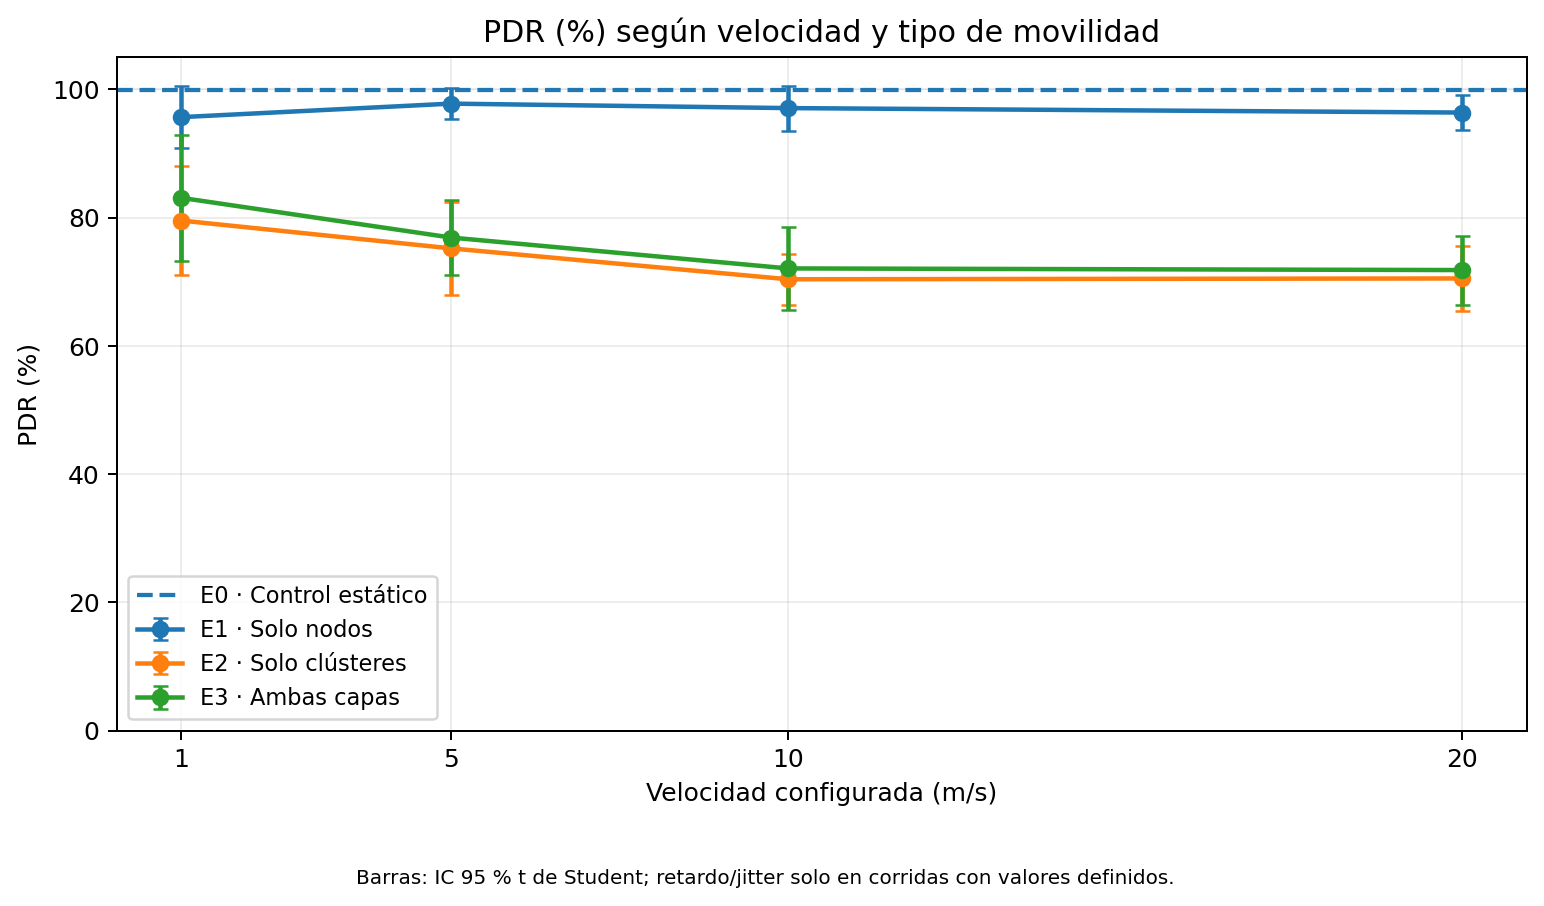
\includegraphics[width=0.95\textwidth]{resultados/figuras/01_pdr_vs_velocidad.png}
\caption{PDR media frente a la velocidad, con intervalos de confianza del 95\,\%. La línea
discontinua es el control E0.}
\label{fig:pdr}
\end{figure}

\begin{figure}[h]
\centering
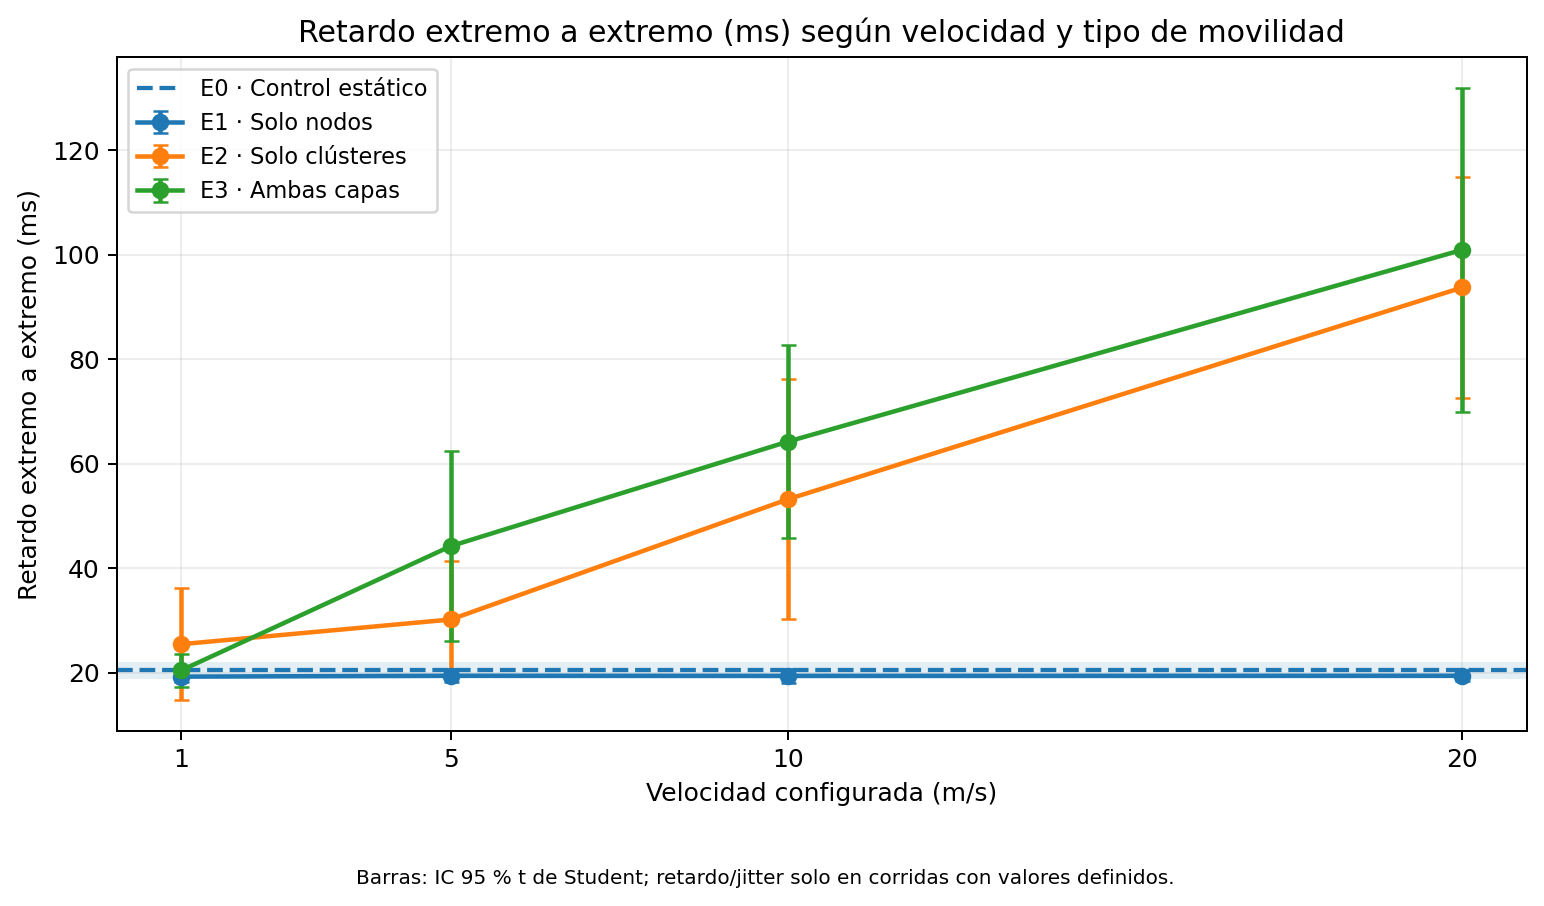
\includegraphics[width=0.95\textwidth]{resultados/figuras/02_retardo_vs_velocidad.png}
\caption{Retardo extremo a extremo medio frente a la velocidad, con intervalos de
confianza del 95\,\%.}
\label{fig:retardo}
\end{figure}

\begin{figure}[h]
\centering
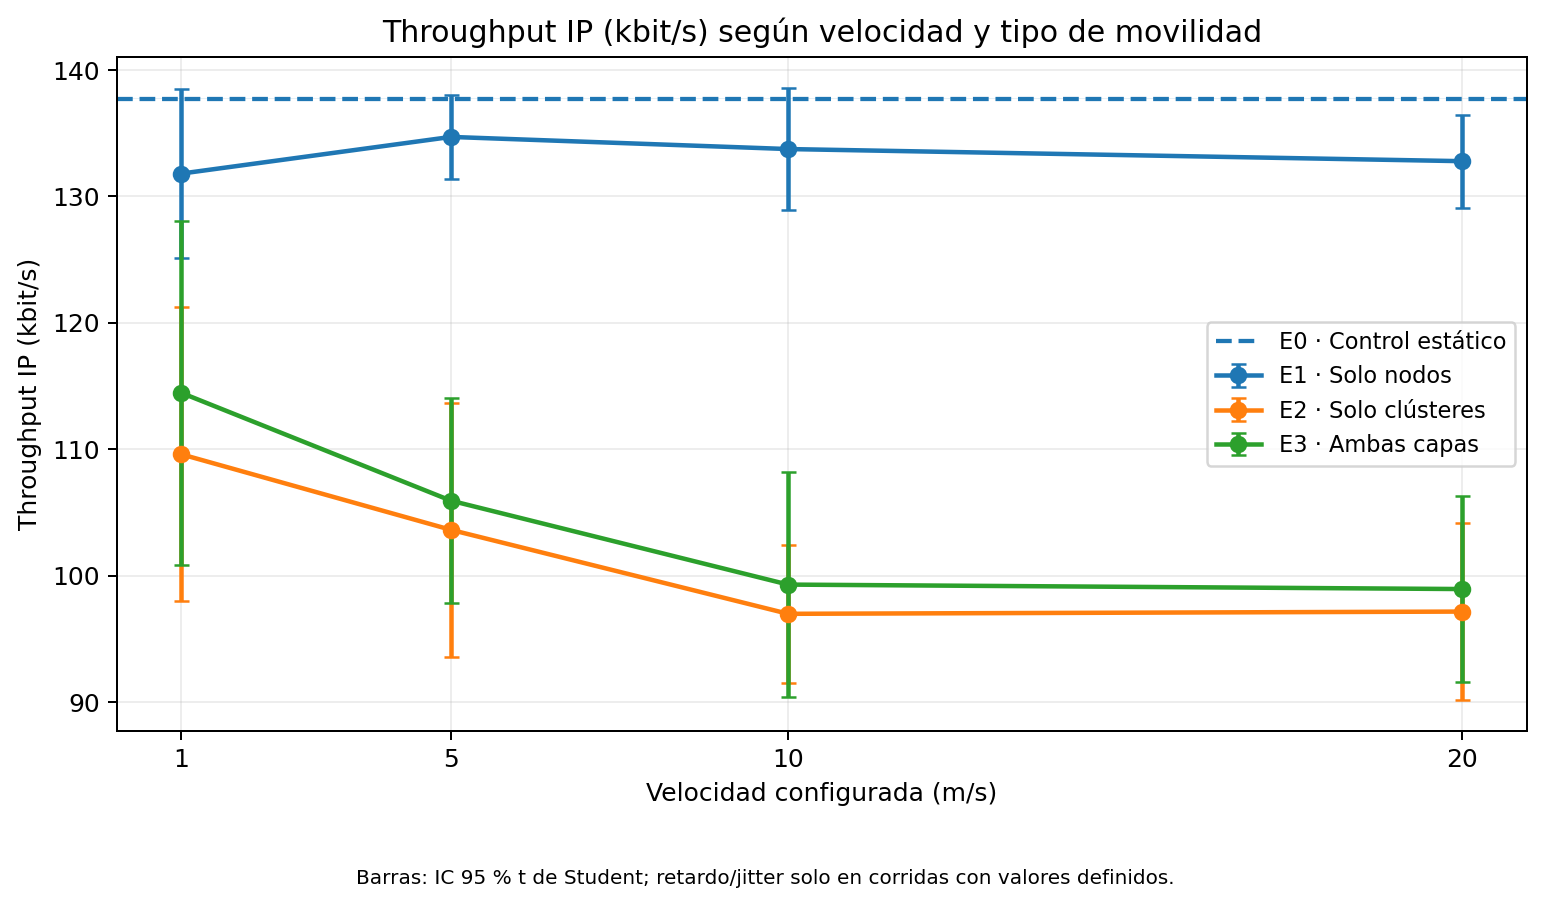
\includegraphics[width=0.48\textwidth]{resultados/figuras/03_throughput_vs_velocidad.png}
\hfill
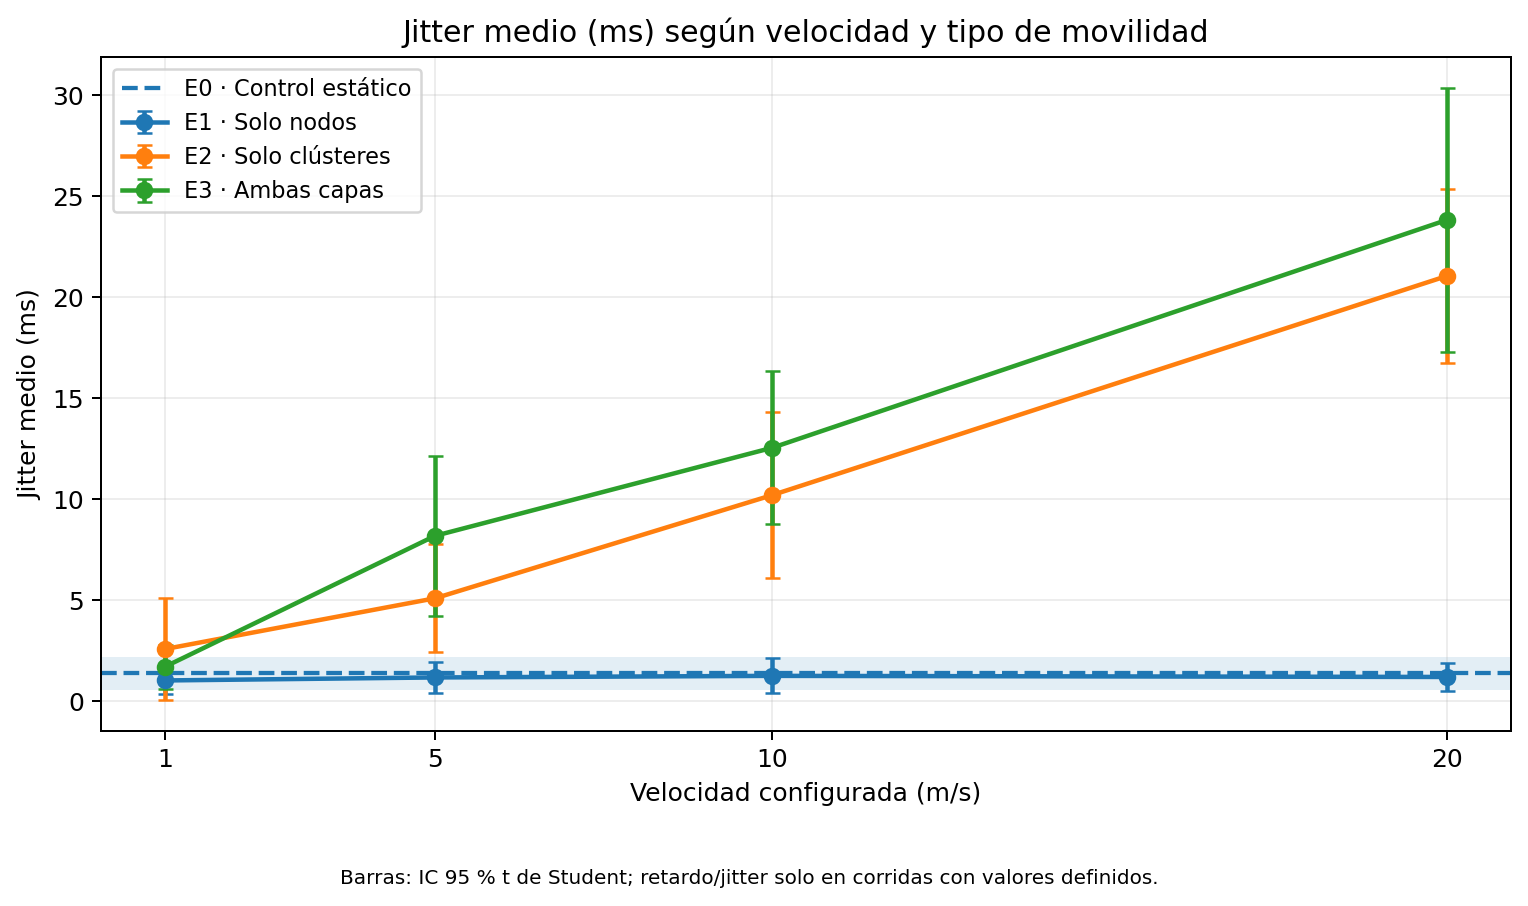
\includegraphics[width=0.48\textwidth]{resultados/figuras/04_jitter_vs_velocidad.png}
\caption{Throughput agregado (izquierda) y jitter medio (derecha) frente a la velocidad.}
\label{fig:throughput-jitter}
\end{figure}

\subsection{Interpretación por escenario}

\textbf{E0 (control).} Sin movilidad la red entrega el 99.97\,\% de los paquetes (mínimo
99.8\,\% entre réplicas), con un retardo de unos 20\,ms. La red está conectada y la
línea base es estable, como exige el diseño (PDR $\geq 95$\,\%). Las pocas pérdidas
corresponden al descubrimiento inicial de rutas de AODV.

\textbf{E1 (solo nodos).} La movilidad de nodo apenas afecta el desempeño: la PDR se
mantiene entre 95.7\,\% y 97.8\,\% y el retardo en unos 19\,ms, prácticamente igual al
control, a cualquier velocidad. Esto se explica por la geometría: un miembro se mueve
como máximo $\pm 40$\,m en cada eje alrededor de su CH, es decir, a lo sumo a
$40\sqrt{2} \approx 56.6$\,m, dentro del alcance de 60\,m del clúster. Los enlaces del
backbone no cambian y el miembro casi siempre tiene un enlace directo con su CH. Las
pérdidas que aparecen (algunas réplicas bajan hasta 78.8\,\%) se deben a rutas locales
de AODV que pasan por otro miembro y se rompen cuando este se aleja.

\textbf{E2 (solo clústeres).} El panorama cambia por completo cuando se mueven los
clústeres. La movilidad de clúster produce la mayor degradación: la
PDR cae a entre 70\,\% y 80\,\% y el retardo crece de 25\,ms a 94\,ms al pasar de 1 a
20\,m/s. Al desplazarse hasta $\pm 150$\,m de su superclúster, dos CH pueden quedar a
más de 250\,m y el backbone se fragmenta: los paquetes entre clústeres se pierden o
esperan en cola mientras AODV busca una ruta nueva. Esa actividad de reparación se
refleja en el número de flujos de control de AODV que registra FlowMonitor, que sube de
17 en E0 a 21 a 1\,m/s y a 55 a 20\,m/s, mientras que en E1 se mantiene en 18--19. La
red, en otras palabras, dedica cada vez más esfuerzo a reconstruir rutas y entrega cada
vez menos.

\textbf{E3 (ambas).} El escenario combinado se comporta como E2: sus medias de PDR
(71.8\,\%--83.1\,\%) y de retardo (20\,ms--101\,ms) no difieren significativamente de las
de E2 a ninguna velocidad (prueba $t$ de Welch bilateral, $p > 0.15$ en las ocho
comparaciones). Sumar la movilidad de nodo a la de clúster no añade una degradación
apreciable.

\subsection{Comparación E1 vs.\ E2: prueba de la hipótesis principal}

La tabla~\ref{tab:welch} presenta las pruebas $t$ de Welch unilaterales
\cite{welch1947generalization} de la hipótesis principal.

\begin{table}[h]
\centering
\small
\begin{tabular}{rlrrrrc}
\toprule
\textbf{$v$} & \textbf{Métrica} & \textbf{E1} & \textbf{E2} & \textbf{$t$} &
\textbf{$p$} & \textbf{¿Rechaza $H_0$?} \\
\midrule
1  & PDR (\%)     & 95.67 & 79.55 & $-3.75$  & 0.0010              & Sí \\
5  & PDR (\%)     & 97.78 & 75.21 & $-6.65$  & $1.8\times10^{-5}$  & Sí \\
10 & PDR (\%)     & 97.08 & 70.39 & $-11.42$ & $<10^{-8}$          & Sí \\
20 & PDR (\%)     & 96.39 & 70.51 & $-10.21$ & $5\times10^{-8}$    & Sí \\
\midrule
1  & Retardo (ms) & 19.2  & 25.4  & 1.31     & 0.111               & No \\
5  & Retardo (ms) & 19.4  & 30.2  & 2.16     & 0.029               & Sí \\
10 & Retardo (ms) & 19.4  & 53.2  & 3.33     & 0.0044              & Sí \\
20 & Retardo (ms) & 19.4  & 93.7  & 7.96     & $1.1\times10^{-5}$  & Sí \\
\bottomrule
\end{tabular}
\caption{Prueba $t$ de Welch unilateral E2 vs.\ E1 por velocidad ($\alpha = 0.05$,
$n = 10$ por grupo). $H_1$: PDR(E2) $<$ PDR(E1) y retardo(E2) $>$ retardo(E1). Fuente:
\texttt{resultados/comparacion\_E2\_vs\_E1.csv}.}
\label{tab:welch}
\end{table}

En PDR se rechaza $H_0$ en las cuatro velocidades, con diferencias de 16 a 27 puntos
porcentuales. En retardo se rechaza en tres de las cuatro: a 1\,m/s el retardo de E2 es
mayor (25.4 frente a 19.2\,ms), pero su alta variabilidad entre réplicas impide que la
diferencia sea significativa. Según la regla de decisión definida de antemano (al menos
tres de cuatro velocidades), \textbf{la hipótesis principal queda respaldada para ambas
métricas}.

\subsection{Efecto de la velocidad e hipótesis secundarias}

\textbf{HS1 (el desempeño empeora con la velocidad).} Se cumple solo cuando hay
movilidad de clúster. En E2 y E3 la PDR a 20\,m/s es significativamente menor que a
1\,m/s ($p = 0.028$ y $p = 0.020$, Welch unilateral) y el retardo se multiplica por
3.7 y 4.9 ($p < 0.001$), con una correlación de Spearman entre velocidad y retardo de
0.76 y 0.81. En E1, en cambio, ni la PDR ni el retardo cambian con la velocidad
($\rho \approx 0$, $p > 0.4$). HS1 queda \textbf{parcialmente respaldada}.

Cabe notar que en E2 y E3 la PDR deja de bajar entre 10 y 20\,m/s (70.4\,\% frente a
70.5\,\% en E2), mientras que el retardo y el jitter siguen creciendo. Una explicación es
que la fracción del tiempo en que el backbone está partido depende sobre todo de la
geometría (dónde están los clústeres), no de la velocidad; la velocidad cambia, en
cambio, la frecuencia con que se rompen y reconstruyen las rutas, que es lo que aumenta
el retardo. A esto se suma una propiedad conocida de Random Waypoint
\cite{yoon2003harmful}: como la pausa de 2\,s es fija, a mayor velocidad los clústeres
pasan más tiempo detenidos (cerca del 4\,\% del tiempo a 1\,m/s y del 21\,\% a 20\,m/s,
medido en la validación), por lo que su velocidad media efectiva es menor que la
configurada.

\textbf{HS2 (E3 igual o peor que el peor de E1 y E2).} El peor escenario individual es
siempre E2, y E3 no difiere significativamente de él en ninguna velocidad. HS2
\textbf{se respalda en su forma ``igual''}: el efecto combinado no es aditivo y está
dominado por la movilidad de clúster.

\textbf{HS3 (la diferencia entre E1 y E2 crece con la velocidad).} La diferencia de
retardo crece de forma monótona (6.2, 10.8, 33.8 y 74.3\,ms a 1, 5, 10 y 20\,m/s). La
diferencia de PDR crece de 16.1 a 26.7 puntos entre 1 y 10\,m/s y luego se estabiliza
(25.9 puntos a 20\,m/s). HS3 queda \textbf{respaldada para el retardo y parcialmente
para la PDR}.
